% !TEX root = ../../thesis.tex
%______________________________________________________________________________
%
% SECTION
\section{Results}
\label{section:results}
%
%______________________________________________________________________________

In this section, the spectral cell method is applied on a simple problem described in \ref{section:error_calculation} with different discretizations and embeddings, and then to an example with a more complex geometry that has a cell distribution more resembling a practical application. For the simple case, approaches without lumping, with density scaling, and with HRZ lumping are compared. All computations are carried out using a modified version of AdhoC++, an in-house high order finite element method developed at the chair of Computational Modeling and Simulation at the Technical University of Munich.

%______________________________________________________________________________
%
% SUB-SECTION
\subsection{Axis-aligned Bar}
\label{section:axis_aligned_bar}
%
%______________________________________________________________________________

A simple straight bar model introduced in \ref{section:error_calculation} is considered. To allow a fictitious domain extension and analyze the behaviour of the SCM, the problem is modeled in 3D instead of one.

\begin{figure}[!h]
	\centering
	\includegraphics[height=3.5cm]{figures/bar_axis_aligned}
	\caption{Embedded axis-aligned bar and its discretization.}
	\label{fig:bar_axis_aligned}
\end{figure}

A bar of length $L_x$ with a rectangular cross-section $L_y \times L_z$ is symmetrically embedded into a Cartesian domain of size $L_x \times 2h_y \times L_z$ that does not conform to the bar in $y$-direction. The domain is discretized by an $n_x \times 2 \times 1$ Cartesian grid of identical cells.

The distributed source defined in equation \ref{eq:toy_problem_source} is extended to 3D but only in the physical domain:

\begin{equation} \label{eq:axis_aligned_source}
	f(\mathbf x,t) = \begin{cases}
	e^{-10^4x^2} sin \left( \frac{2 \pi}{T} t \right) & t \in \left[ 0,\frac{T}{2} \right], \ \mathbf x \in \Omega_p \\[0.5em]
	0 & \text{otherwise} \\
	\end{cases}
\end{equation}

\begin{table}[h]
	\centering
	\bgroup
	\def\arraystretch{1.5}
	\begin{tabular}{|c|c|c|c|c|c|c|c|}
		\hline
		\multicolumn{3}{|c}{geometry} & \multicolumn{2}{|c}{material} & \multicolumn{1}{|c}{source} & \multicolumn{2}{|c|}{time} \\
		\hline \hline
		$L_x$ & $h_y$ & $L_z$ & $\rho$ & $E$ & $T$ & $\Delta t$ & $t_{max}$ \\
		\hline
		$0.5$ & $0.01$ & $0.01$ & $1$ & $1$ & $0.1$ & $2\cdot 10^{-4}$ & $0.5$ \\
		\hline
	\end{tabular}
	\egroup
	\caption{Constant parameters for the bar example.}
\end{table}

Time integration is performed using central differences described in \ref{subsection:wave_equation_temporal_discretization} for every case. In the following subsections, the behaviour of solutions obtained by different approaches is studied, depending on various quantities such as the:

\begin{tabular}{>{\textbullet\hspace{\labelsep}}lr}
	number of elements in $x$-direction & $n_x$ \\
	order of basis functions & $p$ \\
	fill ratio of cells & $\eta$ \\
	fictitious exponent & $\beta$
\end{tabular}\bigskip

%______________________________________________________________________________
% SUB-SUB-SECTION
\subsubsection*{Fill Ratio}
\label{section:fill_ratio}
%______________________________________________________________________________

Since the mass matrices of uncut cells are inherently diagonal, lumping schemes have no effect on them. However, as the proportion of the physical domain in a cell decreases, the role of lumping becomes more dominant. The fill ratio $\eta$ shows the proportion of the physical domain relative to the total volume of a cell. In the bar example, this is controlled by varying the height $L_y$ of the bar while leaving the mesh untouched to avoid errors originating from element skewness. Hence, the fill ratio can be computed as follows:

\begin{equation} \label{eq:fill_ratio}
	\eta = \cfrac{L_y}{2h_y}
\end{equation}

This value is identical for every cell in the model. To make sure that no errors originate from the numerical integration's adaptive nature, the bar's height is always set such that an octree of depth $r$ can perfectly capture its boundary. More precisely, the bar is shrunk sequentially by powers of two: $L_y = 2 ^{-r} \ 2h_y$

\begin{center}
\begin{minipage}[b]{0.45\textwidth}
	\centering
	\bgroup
		\def\arraystretch{2.5}
		\begin{tabular}{|c||c|c|c|c|c|}
			\hline
			$r$ & 0 & 1 & 2 & 3 & 4 \\
			\hline
			$L_y$ & $2h_y$ & $h_y$ & $\cfrac{h_y}{2}$ & $\cfrac{h_y}{4}$ & $\cfrac{h_y}{8}$ \\ 
			\hline
			$\eta$ & $1$ & $\cfrac{1}{2}$ & $\cfrac{1}{4}$ & $\cfrac{1}{8}$ & $\cfrac{1}{16}$ \\
			\hline
		\end{tabular}
	\captionof{table}{Cell fill ratios for different bar heights.}
	\egroup
\end{minipage}
\hfill
\begin{minipage}[b]{0.45\textwidth}
	\centering
	\includegraphics[width=0.75\textwidth]{figures/cell_fill_ratio}
	\captionof{figure}{Example bottom left cell for different bar heights.}
\end{minipage}
\end{center}

For all following cases, the number of elements in $x$-direction $n_x=30$ is fixed and p-refinement is performed $p=1,...,4$. The indicator function $\alpha(\mathbf x)$ is characterized by the fictitious exponent $\beta = 5$. Displacements are evaluated at two sample points defined in section \ref{section:error_calculation}, and the relative error defined in equation \ref{eq:time_of_flight_relative_error} is computed using wavelet peaks.

Note, that the mesh conforms to the boundary for $r=0$, which means that no adaptive integration or lumping is performed, and the solution is identical to that of the standard SEM. This case can be used as reference.

Without lumping, the solutions shown in figure \ref{fig:aligned_bar_fill_ratio_convergence_no_lumping} converge as expected. Spurious oscillations decay as $p$ increases and the effective wave speed approaches the analytical one. The fill ratio has little impact on the results of embedded setups, but the boundary-conforming case visibly differs from them. This is due to the fact that the boundary-conforming case consists of uncut cells whose mass matrices are integrated using Lobatto quadrature, and are therefore underintegrated. On the other hand, cut cells in the non-conforming cases are exactly integrated using the adaptive scheme based on Gauss-Legendre quadrature.
Since no lumping is performed, the mass matrix has non-zero off-diagonal entries from the adaptive integration, thus leading to less efficient time integration.

\begin{figure}[!h]
	\centering
	\includegraphics[height=6cm]{inkscape/fill_ratio_no_lumping/convergence}
	\caption{Relative time-of-flight error for p-refinement on different fill ratios without lumping. The embedded cases $r \neq 0$ overlap within line width.}
	\label{fig:aligned_bar_fill_ratio_convergence_no_lumping}
\end{figure}

\begin{figure}[!h]
	\centering
	\begin{subfigure}[b]{0.49\textwidth}
		\centering
		\raisebox{-\height}{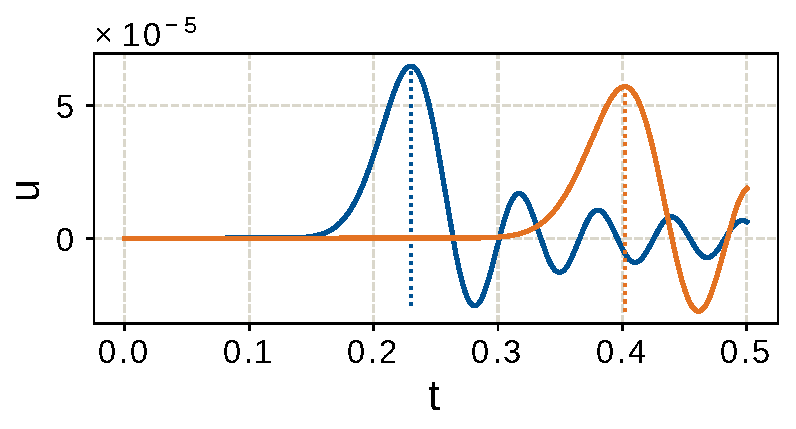
\includegraphics[width=\textwidth]{inkscape/fill_ratio_no_lumping/r0_p1}}
		\caption{$r=0 \ \ \ \ p=1$}
	\end{subfigure}
	\hfill
	\begin{subfigure}[b]{0.49\textwidth}
		\centering
		\raisebox{-\height}{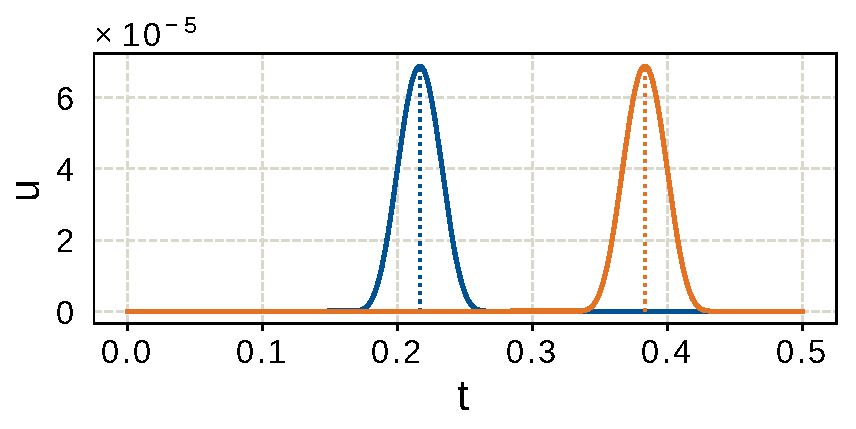
\includegraphics[width=\textwidth]{inkscape/fill_ratio_no_lumping/r0_p4}}
		\caption{$r=0 \ \ \ \ p=4$}
	\end{subfigure}
	\vskip\baselineskip
	\begin{subfigure}[b]{0.49\textwidth}
		\centering
		\raisebox{-\height}{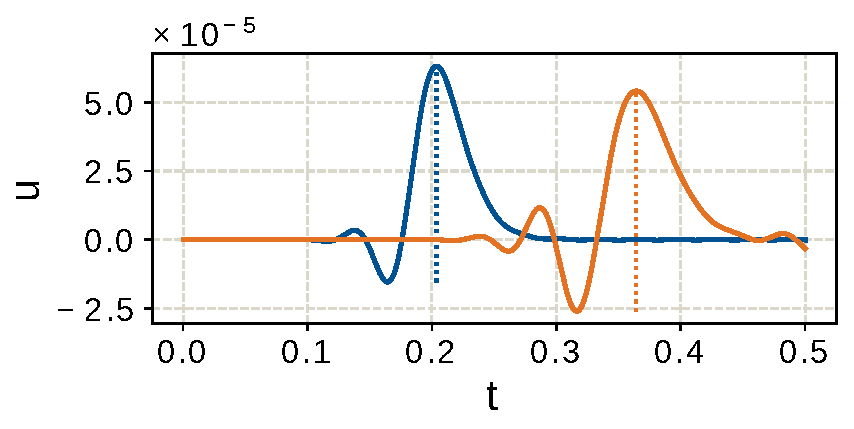
\includegraphics[width=\textwidth]{inkscape/fill_ratio_no_lumping/r4_p1}}
		\caption{$r=4 \ \ \ \ p=1$}
	\end{subfigure}
	\hfill
	\begin{subfigure}[b]{0.49\textwidth}
		\centering
		\raisebox{-\height}{\includegraphics[width=\textwidth]{inkscape/fill_ratio_no_lumping/r4_p4}}
		\caption{$r=4 \ \ \ \ p=4$}
	\end{subfigure}
	\begin{subfigure}[b]{0.49\textwidth}
		\centering
		\raisebox{-\height}{\includegraphics[width=\textwidth]{inkscape/fill_ratio_no_lumping/legend}}
	\end{subfigure}
	\caption{Displacement history at the two points for $r = \{0,4\}$, $p = \{1,4\}$ and no lumping.}
	\label{fig:aligned_bar_fill_ratio_displacement_no_lumping}
\end{figure}

Next, HRZ lumping is applied to the same scenarios. As seen in figure \ref{fig:aligned_bar_fill_ratio_convergence_hrz}, this method is unable to consistently benefit from p-refinement and does not converge in general. To gain a better understanding of why this is the case, the displacements at the two sample points and then on the entire model are studied.

\begin{figure}[!h]
	\centering
	\includegraphics[height=6cm]{inkscape/fill_ratio_hrz/convergence}
	\caption{Relative time-of-flight error for p-refinement on different fill ratios with HRZ lumping.}
	\label{fig:aligned_bar_fill_ratio_convergence_hrz}
\end{figure}

Figure \ref{fig:aligned_bar_fill_ratio_displacement_hrz} shows the displacement histories at the two sample points for a fill ratio of $\eta=\frac{1}{2}$ with $p$ ranging from 1 to 4. At first, increasing the order of the basis seem to attenuate the magnitude of spurious oscillations, but at higher orders this trend is clearly disproven. An interesting observation is that the oscillations occur exclusively after the main wavelet, and resemble decaying harmonic functions. Their source can be better understood by studying how the displacement field changes over time.

\begin{figure}[!h]
	\centering
	\begin{subfigure}[b]{0.49\textwidth}
		\centering
		\raisebox{-\height}{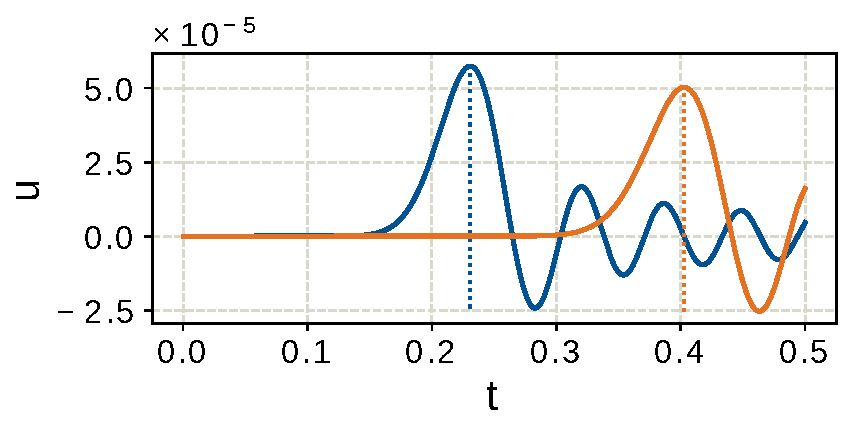
\includegraphics[width=\textwidth]{inkscape/fill_ratio_hrz/r1_p1}}
		\caption{$r=1 \ \ \ \ p=1$}
	\end{subfigure}
	\hfill
	\begin{subfigure}[b]{0.49\textwidth}
		\centering
		\raisebox{-\height}{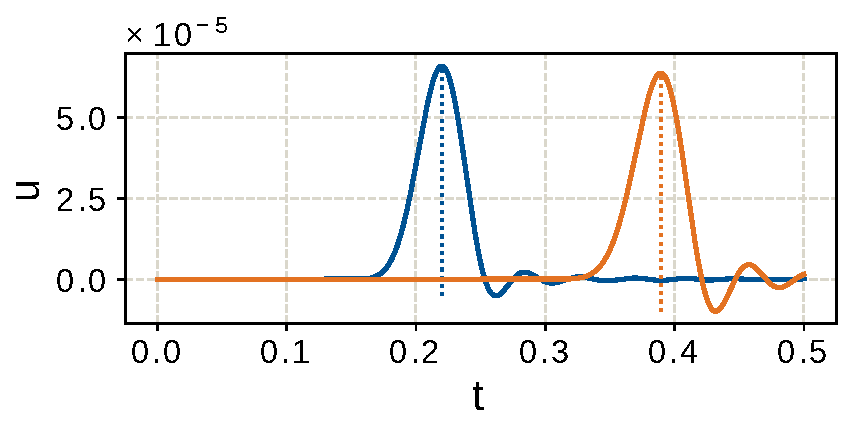
\includegraphics[width=\textwidth]{inkscape/fill_ratio_hrz/r1_p2}}
		\caption{$r=1 \ \ \ \ p=2$}
	\end{subfigure}
	\vskip\baselineskip
	\begin{subfigure}[b]{0.49\textwidth}
		\centering
		\raisebox{-\height}{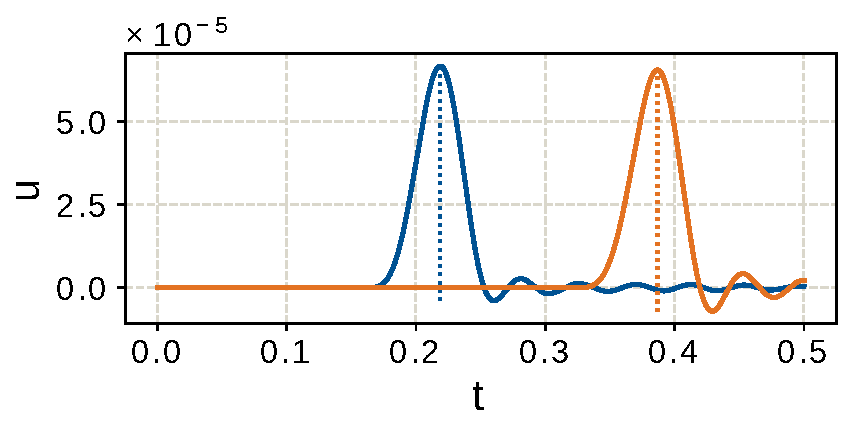
\includegraphics[width=\textwidth]{inkscape/fill_ratio_hrz/r1_p3}}
		\caption{$r=1 \ \ \ \ p=3$}
	\end{subfigure}
	\hfill
	\begin{subfigure}[b]{0.49\textwidth}
		\centering
		\raisebox{-\height}{\includegraphics[width=\textwidth]{inkscape/fill_ratio_hrz/r1_p4}}
		\caption{$r=1 \ \ \ \ p=4$}
		\label{fig:aligned_bar_fill_ratio_displacement_hrz_r1_p4}
	\end{subfigure}
	\begin{subfigure}[b]{0.49\textwidth}
		\centering
		\raisebox{-\height}{\includegraphics[width=\textwidth]{inkscape/fill_ratio_no_lumping/legend}}
	\end{subfigure}
	\caption{Displacement history at the two points for $r=1$, $p \in \{1,...,4\}$ and HRZ lumping.}
	\label{fig:aligned_bar_fill_ratio_displacement_hrz}
\end{figure}

Figure \ref{fig:fill_ratio_hrz_displacement_field} compares the displacement field with HRZ lumping to the solution without lumping at different time points, for the setup $r=1$ and $p=4$. The solution without lumping can be regarded as reference, and as expected, the displacement is constant in $y$-direction, even in the fictitious domain. The wavelet propagates in the $x$-direction without skewing, and no reflections occur on the boundary between the physical and fictitious domains. 
In contrast, HRZ lumping introduces a variance in the $y$-direction. It is important to note that for better visibility, the displacement color range is adjusted for magnitudes in the physical domain $\pm 7\cdot 10^{-5}$, but this range is almost an order of magnitude greater in the fictitious domain $\pm 2.5 \cdot 10^{-4}$.
Furthermore, the wave speed appears to differ in $\Omega_f$ which leads to a wave front propagating in $y$-direction, endlessly reflected between the boundary of the domains and the mesh. 
In the FCM, the displacement magnitudes in $\Omega_f$ must be at least in the order of $10^{\beta}$ greater than the solution of the physical domain to have notable effect on it.
Due to the artificial coupling between the physical and fictitious domains introduced by HRZ lumping however, the waves originating from $\Omega_f$ propagate into the physical domain as well, albeit with reduced amplitude. The resulting spurious oscillations can be clearly observed in the displacement history of the sample points as well, shown in figure \ref{fig:aligned_bar_fill_ratio_displacement_hrz_r1_p4}. Their magnitude, frequency, and phase relative to wavelet depend on the size of the fictitious domain and the material properties inside it, defined by $\beta$.

\begin{figure}[!h]
	\centering
	\begin{subfigure}[b]{0.45\textwidth}
		\centering
		\raisebox{-\height}{\includegraphics[width=\textwidth]{figures/paraview_aligned_hrz/animation.0001}}
	\end{subfigure}
	\hfill
	\begin{subfigure}[b]{0.45\textwidth}
		\centering
		\raisebox{-\height}{\includegraphics[width=\textwidth]{figures/paraview_aligned_none/animation.0001}}
	\end{subfigure}
	\vskip \baselineskip
	\begin{subfigure}[b]{0.45\textwidth}
		\centering
		\raisebox{-\height}{\includegraphics[width=\textwidth]{figures/paraview_aligned_hrz/animation.0002}}
	\end{subfigure}
	\hfill
	\begin{subfigure}[b]{0.45\textwidth}
		\centering
		\raisebox{-\height}{\includegraphics[width=\textwidth]{figures/paraview_aligned_none/animation.0002}}
	\end{subfigure}
	\vskip \baselineskip
	\begin{subfigure}[b]{0.45\textwidth}
		\centering
		\raisebox{-\height}{\includegraphics[width=\textwidth]{figures/paraview_aligned_hrz/animation.0003}}
	\end{subfigure}
	\hfill
	\begin{subfigure}[b]{0.45\textwidth}
		\centering
		\raisebox{-\height}{\includegraphics[width=\textwidth]{figures/paraview_aligned_none/animation.0003}}
	\end{subfigure}
	\vskip \baselineskip
	\begin{subfigure}[b]{0.45\textwidth}
		\centering
		\raisebox{-\height}{\includegraphics[width=\textwidth]{figures/paraview_aligned_hrz/animation.0004}}
	\end{subfigure}
	\hfill
	\begin{subfigure}[b]{0.45\textwidth}
		\centering
		\raisebox{-\height}{\includegraphics[width=\textwidth]{figures/paraview_aligned_none/animation.0004}}
	\end{subfigure}
	\vskip \baselineskip
	\begin{subfigure}[b]{0.45\textwidth}
		\centering
		\raisebox{-\height}{\includegraphics[width=\textwidth]{figures/paraview_aligned_hrz/animation.0005}}
		\caption{HRZ lumping}
	\end{subfigure}
	\hfill
	\begin{subfigure}[b]{0.45\textwidth}
		\centering
		\raisebox{-\height}{\includegraphics[width=\textwidth]{figures/paraview_aligned_none/animation.0005}}
		\caption{no lumping}
	\end{subfigure}
	\begin{subfigure}[b]{0.95\textwidth}
		\centering
		\includegraphics[width=0.65\textwidth]{figures/paraview_aligned_hrz/legend}
	\end{subfigure}
	\caption{Cropped top view of the displacement field at $t=\{0.04, \ 0.08, \ 0.12, \ 0.16, \ 0.2\}$ with HRZ lumping (left) and without lumping (right). The fill ratio $\eta=\frac{1}{2}$ and basis order $p=4$ is identical for both cases.}
	\label{fig:fill_ratio_hrz_displacement_field}
\end{figure}

In an attempt to dispose of the solution's variance in y-direction, a model with the source term $f$ extended to the fictitious domain and multiplied by the indicator function $\alpha$ was studied as well, but yielded similar results.

Finally, density scaling is studied for the same setup. Considering that it similar to HRZ lumping but with more simplifications, the fact that it performs worse is not surprising. However, an interesting property can be observed in the displacement histories that may help better understand why neither lumping schemes are viable. Originally, both the density $\rho$ and Young's modulus $E$ are multiplied by $10^{-\beta}$ in the fictitious domain, which means that the wave speed remains constant over the entirety of the model. As mentioned in \ref{subsection:density_scaling_lumping} however, density scaling imposes a uniform mass distribution on cut cells. Apart from introducing an artificial coupling between domains similar to HRZ lumping, this means that the effective wave speed becomes higher in the physical domain while lower in the fictitious one. Furthermore, this speed difference varies from cell to cell, depending on their individual fill ratios. Though combined with other errors, this behaviour can be seen in figure \ref{fig:aligned_bar_fill_ratio_displacement_density_scaling}. As the fill ratio decreases, the propagating wavelet becomes faster in the physical domain. For fill ratios of $\eta=\frac{1}{8}$ and $\eta=\frac{1}{16}$, the wave is reflected from the right boundary and even reaches $P_2$ on its way back before $t_{max}$.

\begin{figure}[!h]
	\centering
	\includegraphics[height=5cm]{inkscape/fill_ratio_density_scaling/convergence}
	\caption{Relative time-of-flight error for p-refinement on different fill ratios with density scaling.}
	\label{fig:aligned_bar_fill_ratio_convergence_density_scaling}
\end{figure}

\begin{figure}[!h]
	\centering
	\begin{subfigure}[b]{0.49\textwidth}
		\centering
		\raisebox{-\height}{\includegraphics[width=\textwidth]{inkscape/fill_ratio_density_scaling/r1_p4}}
		\caption{$r=1 \ \ \ \ p=4$}
	\end{subfigure}
	\hfill
	\begin{subfigure}[b]{0.49\textwidth}
		\centering
		\raisebox{-\height}{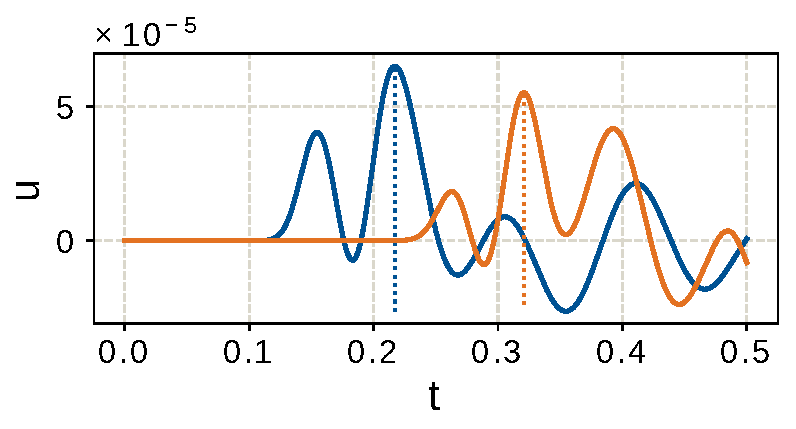
\includegraphics[width=\textwidth]{inkscape/fill_ratio_density_scaling/r2_p4}}
		\caption{$r=2 \ \ \ \ p=4$}
	\end{subfigure}
	\vskip\baselineskip
	\begin{subfigure}[b]{0.49\textwidth}
		\centering
		\raisebox{-\height}{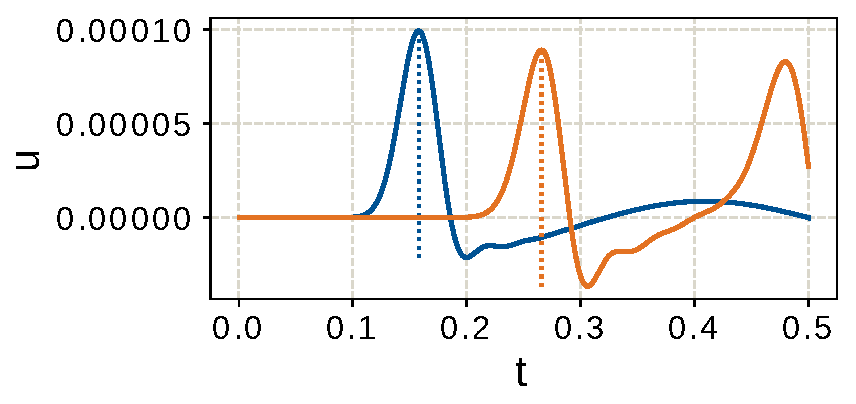
\includegraphics[width=\textwidth]{inkscape/fill_ratio_density_scaling/r3_p4}}
		\caption{$r=3 \ \ \ \ p=4$}
	\end{subfigure}
	\hfill
	\begin{subfigure}[b]{0.49\textwidth}
		\centering
		\raisebox{-\height}{\includegraphics[width=\textwidth]{inkscape/fill_ratio_density_scaling/r4_p4}}
		\caption{$r=4 \ \ \ \ p=4$}
	\end{subfigure}
	\begin{subfigure}[b]{0.49\textwidth}
		\centering
		\raisebox{-\height}{\includegraphics[width=\textwidth]{inkscape/fill_ratio_density_scaling/legend}}
	\end{subfigure}
	\caption{Displacement history at the two points for $r \in \{1,...,4\}$, $p = 4$ and density scaling.}
	\label{fig:aligned_bar_fill_ratio_displacement_density_scaling}
\end{figure}

In conclusion, neither lumping schemes are viable. An interesting property of both methods is that due to the artificially coupled domains, the magnitude, frequency, and phase of the spurious oscillations vary with $\eta$ and $p$. To show how important and non-trivial the impact the displacement in the fictitious domain has on the physical one, the solution's dependence on the fictitious exponent $\beta$ is analyzed in the next section. As density scaling is similar to HRZ lumping but clearly inferior, it is not studied in the rest of this thesis.

%______________________________________________________________________________
% SUB-SUB-SECTION
\subsubsection*{Fictitious Exponent}
\label{section:fictitious_exponent}
%______________________________________________________________________________

Introduced in equation \ref{eq:indicator_function}, the fictitious exponent $\beta$ defines the relation between the material parameters in the physical and fictitious domains. Its original purpose in the FCM is to avoid ill conditioned structural matrices for badly cut cells. Small values lead to more stable numerics but less accurate physics, thus one has to find an acceptable compromise between the two types of errors. That said, there is no detailed study on its effect, and its value is often arbitrarily chosen between 3 and 10 \cite{Parvizian2007}. Due to lumping however, the solution in the fictitious domain has a greater impact, making $\beta$ more important in the SCM.

In the following examples, the fill ratio $\eta = \frac{1}{4}$ and basis order $p=4$ remain constant while the $\beta$ varies between 0 and 10. Since the focus is on the residual oscillations in this case, the time of arrival is computed based on the envelope of the displacement history. The specifics of this process and reason for doing so are discussed in \ref{section:error_calculation}.

Figure \ref{fig:beta_convergence} shows how the resulting error changes with the fictitious exponent. At $\beta = 0$, the material in the two domains are identical, thus the stiffness and mass matrices are consistent. Lumping has minimal effect, and no oscillations occur in this case. In the range $\beta \in [2,\ 6]$ however, oscillations appear and vary in magnitude, frequency, and phase.

The source of these oscillations in the fictitious domain and their varying wavelengths can be observed in figure \ref{fig:hrz_displacement_field_beta}, which compares the displacement fields progress over time for $\beta=3.5$ and $\beta=4.5$. Note, that unlike in figure \ref{fig:fill_ratio_hrz_displacement_field}, the color scale covers the entirety of the displacement magnitude in this case, in order to focus on the fictitious domain.

\begin{figure}[!h]
	\centering
	\includegraphics[height=4.5cm]{inkscape/beta/convergence}
	\caption{Relative time-of-flight error for varying fictitious exponents $\beta$.}
	\label{fig:beta_convergence}
\end{figure}

\begin{figure}[!h]
	\centering
	\begin{subfigure}[b]{0.49\textwidth}
		\centering
		\raisebox{-\height}{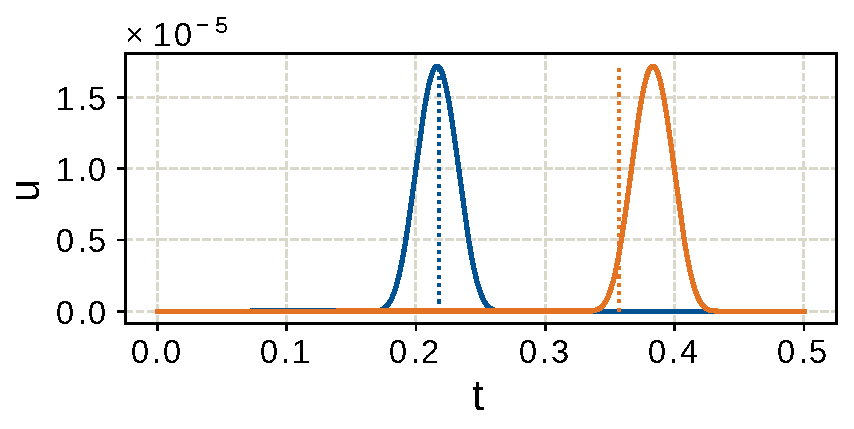
\includegraphics[width=\textwidth]{inkscape/beta/beta_0.0}}
		\caption{$\beta=0$}
	\end{subfigure}
	\hfill
	\begin{subfigure}[b]{0.49\textwidth}
		\centering
		\raisebox{-\height}{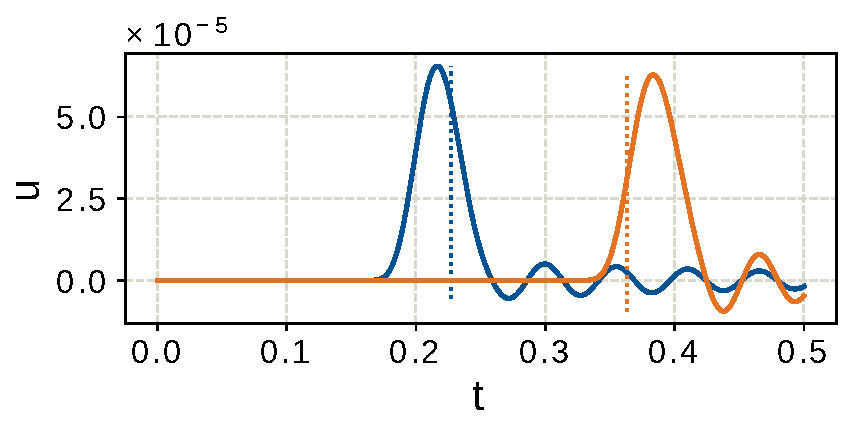
\includegraphics[width=\textwidth]{inkscape/beta/beta_3.5}}
		\caption{$\beta=3.5$}
	\end{subfigure}
	\vskip\baselineskip
	\begin{subfigure}[b]{0.49\textwidth}
		\centering
		\raisebox{-\height}{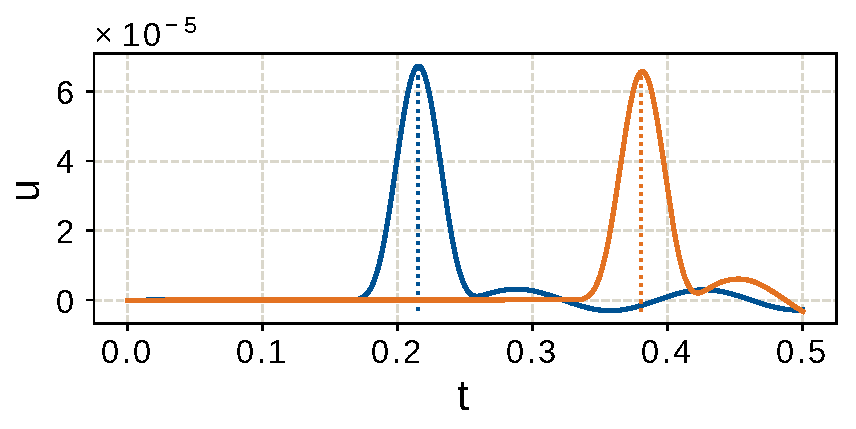
\includegraphics[width=\textwidth]{inkscape/beta/beta_4.5}}
		\caption{$\beta=4.5$}
	\end{subfigure}
	\hfill
	\begin{subfigure}[b]{0.49\textwidth}
		\centering
		\raisebox{-\height}{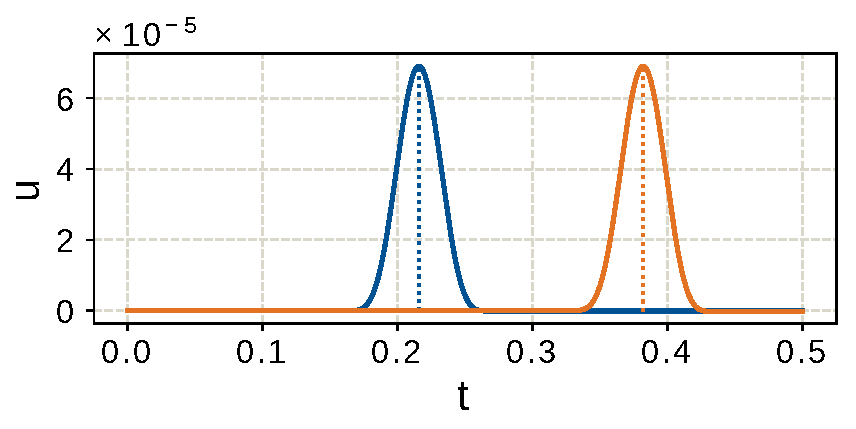
\includegraphics[width=\textwidth]{inkscape/beta/beta_10.0}}
		\caption{$\beta=10$}
	\end{subfigure}
	\begin{subfigure}[b]{0.49\textwidth}
		\centering
		\raisebox{-\height}{\includegraphics[width=\textwidth]{inkscape/beta/legend}}
	\end{subfigure}
	\caption{Displacement history at the two points for $\eta=\frac{1}{4}$, $p = 4$ and HRZ lumping.}
	\label{fig:aligned_bar_displacement_beta}
\end{figure}

\begin{figure}[!h]
	\centering
	\begin{subfigure}[b]{0.45\textwidth}
		\centering
		\raisebox{-\height}{\includegraphics[width=\textwidth]{figures/paraview_aligned_beta_3.5/animation.0001}}
	\end{subfigure}
	\hfill
	\begin{subfigure}[b]{0.45\textwidth}
		\centering
		\raisebox{-\height}{\includegraphics[width=\textwidth]{figures/paraview_aligned_beta_4.5/animation.0001}}
	\end{subfigure}
	\vskip \baselineskip
	\begin{subfigure}[b]{0.45\textwidth}
		\centering
		\raisebox{-\height}{\includegraphics[width=\textwidth]{figures/paraview_aligned_beta_3.5/animation.0002}}
	\end{subfigure}
	\hfill
	\begin{subfigure}[b]{0.45\textwidth}
		\centering
		\raisebox{-\height}{\includegraphics[width=\textwidth]{figures/paraview_aligned_beta_4.5/animation.0002}}
	\end{subfigure}
	\vskip \baselineskip
	\begin{subfigure}[b]{0.45\textwidth}
		\centering
		\raisebox{-\height}{\includegraphics[width=\textwidth]{figures/paraview_aligned_beta_3.5/animation.0003}}
	\end{subfigure}
	\hfill
	\begin{subfigure}[b]{0.45\textwidth}
		\centering
		\raisebox{-\height}{\includegraphics[width=\textwidth]{figures/paraview_aligned_beta_4.5/animation.0003}}
	\end{subfigure}
	\vskip \baselineskip
	\begin{subfigure}[b]{0.45\textwidth}
		\centering
		\raisebox{-\height}{\includegraphics[width=\textwidth]{figures/paraview_aligned_beta_3.5/animation.0004}}
	\end{subfigure}
	\hfill
	\begin{subfigure}[b]{0.45\textwidth}
		\centering
		\raisebox{-\height}{\includegraphics[width=\textwidth]{figures/paraview_aligned_beta_4.5/animation.0004}}
	\end{subfigure}
	\vskip \baselineskip
	\begin{subfigure}[b]{0.45\textwidth}
		\centering
		\raisebox{-\height}{\includegraphics[width=\textwidth]{figures/paraview_aligned_beta_3.5/animation.0005}}
		\caption{$\beta=3.5$}
	\end{subfigure}
	\hfill
	\begin{subfigure}[b]{0.45\textwidth}
		\centering
		\raisebox{-\height}{\includegraphics[width=\textwidth]{figures/paraview_aligned_beta_4.5/animation.0005}}
		\caption{$\beta=4.5$}
	\end{subfigure}
	\begin{subfigure}[b]{0.95\textwidth}
		\centering
		\includegraphics[width=0.55\textwidth]{figures/paraview_aligned_beta_3.5/legend}
	\end{subfigure}
	\caption{Cropped top view of the displacement field at $t=\{0.04, \ 0.08, \ 0.12, \ 0.16, \ 0.2\}$, $\beta = \{3.5, \ 4.5\}$ with HRZ lumping. The fill ratio $\eta=\frac{1}{4}$ and basis order $p=4$ is identical for both cases.}
	\label{fig:hrz_displacement_field_beta}
\end{figure}

Although for this specific set of configurations, oscillations occur in a range of $\beta$ but disappear completely for $\beta > 6$. The same does not hold true in general, and spurious oscillations persist for large fictitious exponents as well. The only general rule is that no such oscillations can be observed for uniform material parameters ($\beta=0$) and that the behaviour of the solution greatly depends on $\beta$.

%______________________________________________________________________________
%
% SUB-SECTION
\subsection{Rotated Bar}
\label{section:rotated_bar}
%
%______________________________________________________________________________

In this section, the bar is rotated by $45$ degrees relative to the mesh and embedded into a Cartesian domain of size $\frac{L_x + L_y}{\sqrt{2}} \times \frac{L_x + L_y}{\sqrt{2}} \times L_z$, discretized by $30 \times 30 \times 1$ identical cells with a basis order of $p=4$.
The most important difference between the rotated and axis-aligned cases is that the geometry cannot be exactly captured by a standard octree, leading to integration errors. By increasing the octree's depth, this error can be arbitrarily reduced at the expense of an exponential increase in complexity. As a compromise between accuracy and performance, the maximum depth is set to $r=p+1=5$.
All other parameters are identical to the ones used in previous examples.

In practical implementations, cells entirely in the fictitious domain are filtered out as they are not part of the original problem and add superfluous degrees of freedom, increasing the computational load. In this example, the solution in the fictitious domain is also of interest, hence such cells are present in the model as well. The resulting mesh contains uncut cells fully in one of the domains, cells cut roughly in half, and badly cut cells that have a small region of physical domain around one of their corners.

%\begin{figure}[!h]
%	\centering
%	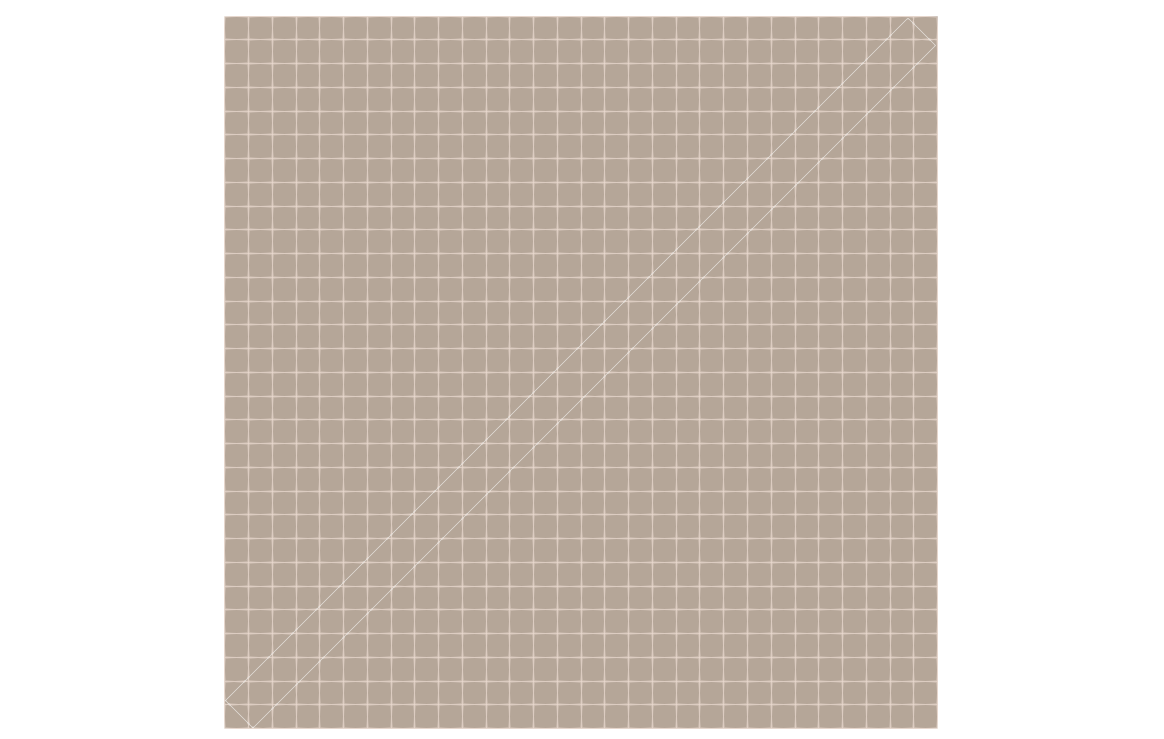
\includegraphics[height=5cm]{figures/paraview_rotated/mesh}
%	\caption{Rotated bar embedded in a Cartesian mesh.}
%	\label{fig:rotated_bar_mesh}
%\end{figure}

\begin{figure}[!h]
	\centering
	\begin{subfigure}[b]{0.49\textwidth}
		\centering
		\raisebox{-\height}{
\includegraphics[width=0.8\textwidth]{figures/paraview_rotated/legend_physical}}
	\end{subfigure}
	\hfill
	\begin{subfigure}[b]{0.49\textwidth}
		\centering
		\raisebox{-\height}{\includegraphics[width=0.8\textwidth]{figures/paraview_rotated/legend_fictitious}}
	\end{subfigure}
	\vskip \baselineskip
	\begin{subfigure}[b]{0.49\textwidth}
		\centering
		\raisebox{-\height}{\includegraphics[width=\textwidth]{figures/paraview_rotated/animation.0002}}
		\caption{$t=0.08$}
	\end{subfigure}
	\hfill
	\begin{subfigure}[b]{0.49\textwidth}
		\centering
		\raisebox{-\height}{\includegraphics[width=\textwidth]{figures/paraview_rotated/animation.0003}}
		\caption{$t=0.12$}
	\end{subfigure}
	\vskip \baselineskip
	\begin{subfigure}[b]{0.49\textwidth}
		\centering
		\raisebox{-\height}{\includegraphics[width=\textwidth]{figures/paraview_rotated/animation.0004}}
		\caption{$t=0.16$}
	\end{subfigure}
	\hfill
	\begin{subfigure}[b]{0.49\textwidth}
		\centering
		\raisebox{-\height}{\includegraphics[width=\textwidth]{figures/paraview_rotated/animation.0005}}
		\caption{$t=0.20$}
	\end{subfigure}
	\caption{Displacement fields of the rotated bar example at different time points. Note, that the physical and fictitious domains have separate ranges and color maps on account of large differences in magnitude.}
\end{figure}

\begin{figure}[!h]
	\centering
	\includegraphics[height=4cm]{figures/paraview_rotated/displacements}
	\caption{Displacement history at the two sample points of the rotated bar.}
	\label{fig:rotated_bar_dislacements}
\end{figure}

Similarly to the axis-aligned cases, spurious oscillations are observed in the physical domain, and the range of displacements in the fictitious domain is roughly an order of magnitude greater. As shown in figure \ref{fig:rotated_bar_extended_cross_section}, the displacement of cut cells sharply increases in magnitude in regions opposite the physical domain. The solution in these areas vary greatly across adjacent cells and oscillate with little decay after the wave passes, disturbing the solution in the physical domain.

\begin{figure}[!h]
	\centering
	\begin{subfigure}{0.49\textwidth}
		\centering
		\raisebox{-\height}{\includegraphics[width=\textwidth]{figures/paraview_rotated/plot_over_line_location}}
	\end{subfigure}
	\hfill
	\begin{subfigure}{0.49\textwidth}
		\centering
		\raisebox{-\height}{\includegraphics[width=\textwidth]{figures/paraview_rotated/plot_over_line}}
	\end{subfigure}
	\caption{Displacement along an extended cross-section of the bar, cutting elements along their diagonals.}
	\label{fig:rotated_bar_extended_cross_section}
\end{figure}

%______________________________________________________________________________
%
% SUB-SECTION
\subsection{Complex Geometry}
\label{section:complex_geometry}
%
%______________________________________________________________________________

The examples so far offered little variety in cell boundary shapes and fill ratios, which may bias the conclusions drawn from their results. To see how the method with HRZ lumping performs in a more practical setting, a geometrically more complex model is studied that provides a variety of fill ratios. The model is similar to the ones before, but instead of a bar, the wavelet is sent down the longest axis of an ellipsoid cut in half, defined as:

\begin{equation} \label{eq:ellipsoid_definition}
	\Omega_p = \left\{
		\mathbf x \left|
			x \leq 1
			\ \ \land \ \
			\left( \cfrac{x-1}{1} \right)^2
			+ \left( \cfrac{y-0.2}{0.2} \right)^2
			+ \left( \cfrac{z-0.1}{0.1} \right)^2
			\leq 1
		\right.
	\right\}
\end{equation}

In order to compensate for the sharp changes in curvature at the tip of the ellipsoid, the source's shape $f_x$ is slightly modified to decay less abruptly:

\begin{equation} \label{eq:ellipsoid_source}
f(\mathbf x,t) = \begin{cases}
e^{-10^3x^2} sin \left( \frac{2 \pi}{T} t \right) & t \in \left[ 0,\frac{T}{2} \right], \ \mathbf x \in \Omega_p \\[0.5em]
0 & \text{otherwise} \\
\end{cases}
\end{equation}

\begin{figure}[!h]
	\centering
	\hspace*{3cm}\includegraphics[height=3.5cm]{figures/paraview_ellipsoid/geometry}
	\caption{Geometry of the physical domain.}
	\label{ref:ellipsoid_geometry}
\end{figure}

The Cartesian embedding domain $\Omega = [0, \ 1] \times [0, \ 0.4] \times [0, \ 0.2]$ is discretized by a $60 \times  24 \times 12$ mesh of cells with a Lagrange basis of order $p=4$. Cells fully in the fictitious domain are neglected. The distribution of cells' fill ratios is shown in figure \ref{fig:ellipsoid_fill_ratio_histogram}, indicating that most cells are uncut and the rest have diverse fill ratios. The mass matrices of uncut cells are integrated with a fifth order Gauss-Lobatto quadrature, while an adaptive scheme with Gauss-Legendre quadrature of identical order is applied to cut cells, then lumped using the HRZ procedure. A reference solution without lumping is computed as well.

\begin{figure}[!h]
	\centering
	\includegraphics[height=5.5cm]{figures/ellipsoid_fill_ratio_histogram}
	\caption{Histogram of the cells' fill ratios.}
	\label{fig:ellipsoid_fill_ratio_histogram}
\end{figure}

Similarly to the bar example, the displacement history is sampled at two points $P_0$ and $P_1$ that trisect the major axis of the half-ellipsoid. Furthermore, a marching cube algorithm is used to recover the geometry's surface and interpolate the solution field on it.

\begin{figure}[!h]
	\centering
	\begin{subfigure}{0.95\textwidth}
		\centering
		\includegraphics[width=0.45\textwidth]{figures/paraview_ellipsoid/displacement_history_legend}
	\end{subfigure}
	%\vfill
	\begin{subfigure}{0.49\textwidth}
		\centering
		\raisebox{-\height}{\includegraphics[width=\textwidth]{figures/paraview_ellipsoid/hrz/displacement_history}}
		\caption{HRZ lumping}
	\end{subfigure}
	\hfill
	\begin{subfigure}{0.49\textwidth}
		\centering
		\raisebox{-\height}{\includegraphics[width=\textwidth]{figures/paraview_ellipsoid/none/displacement_history}}
		\caption{no lumping}
	\end{subfigure}
	\caption{Displacement histories at the two sample points on the ellipsoid's major axis with HRZ lumping (left) and without lumping (right).}
	\label{fig:ellipsoid_displacement_history}
\end{figure}

\begin{figure}[!h]
	\centering
	\begin{subfigure}[b]{0.95\textwidth}
		\centering
		\raisebox{-\height}{\includegraphics[width=0.4\textwidth]{figures/paraview_ellipsoid/legend}}
	\end{subfigure}
	\vskip \baselineskip
	\begin{subfigure}[b]{0.49\textwidth}
		\centering
		\raisebox{-\height}{\includegraphics[width=\textwidth]{figures/paraview_ellipsoid/hrz/animation.0001}}
	\end{subfigure}
	\hfill
	\begin{subfigure}[b]{0.49\textwidth}
		\centering
		\raisebox{-\height}{\includegraphics[width=\textwidth]{figures/paraview_ellipsoid/none/animation.0001}}
	\end{subfigure}
	\vskip\baselineskip
	\begin{subfigure}[b]{0.49\textwidth}
		\centering
		\raisebox{-\height}{\includegraphics[width=\textwidth]{figures/paraview_ellipsoid/hrz/animation.0002}}
	\end{subfigure}
	\hfill
	\begin{subfigure}[b]{0.49\textwidth}
		\centering
		\raisebox{-\height}{\includegraphics[width=\textwidth]{figures/paraview_ellipsoid/none/animation.0002}}
	\end{subfigure}
	\vskip\baselineskip
	\begin{subfigure}[b]{0.49\textwidth}
		\centering
		\raisebox{-\height}{\includegraphics[width=\textwidth]{figures/paraview_ellipsoid/hrz/animation.0003}}
	\end{subfigure}
	\hfill
	\begin{subfigure}[b]{0.49\textwidth}
		\centering
		\raisebox{-\height}{\includegraphics[width=\textwidth]{figures/paraview_ellipsoid/none/animation.0003}}
	\end{subfigure}
	\vskip\baselineskip
	\begin{subfigure}[b]{0.49\textwidth}
		\centering
		\raisebox{-\height}{\includegraphics[width=\textwidth]{figures/paraview_ellipsoid/hrz/animation.0004}}
		\caption{HRZ lumping}
	\end{subfigure}
	\hfill
	\begin{subfigure}[b]{0.49\textwidth}
		\centering
		\raisebox{-\height}{\includegraphics[width=\textwidth]{figures/paraview_ellipsoid/none/animation.0004}}
		\caption{no lumping}
	\end{subfigure}
	\caption{Displacement fields on the surface of the ellipsoid at $t=\{0.2, \ 0.4, \ 0.6, \ 0.8\}$, computed with HRZ lumping (left) and no lumping as reference (right).}
	\label{fig:ellipsoid_surface_displacement}
\end{figure}

As figure \ref{fig:ellipsoid_displacement_history} shows, the spurious oscillations originating from cut cells are similar to the ones in the bar examples, and are superposed on the reference solution. However, their influence is more modest due to relatively smaller element sizes, and fewer cut cells compared to uncut ones. Figure \ref{fig:ellipsoid_cross_section} shows the displacement history on the cross-section at $P_0$ between $t \in [0.67, \ 0.82]$, well after the wavelet passed. The solution in the fictitious domain is seen to persistently oscillate, even without notable excitation coming from the physical domain.

In conclusion, the errors introduced by HRZ lumping are similar to earlier results and are still unacceptable even though the mesh mainly consists of uncut cells.

\begin{figure}[!h]
	\centering
	\begin{subfigure}[b]{0.95\textwidth}
		\centering
		\raisebox{-\height}{\includegraphics[width=0.4\textwidth]{figures/paraview_ellipsoid/cross_section/legend}}
	\end{subfigure}
	\begin{subfigure}[b]{0.24\textwidth}
		\centering
		\raisebox{-\height}{\includegraphics[width=\textwidth]{figures/paraview_ellipsoid/cross_section/animation.0067}}
	\end{subfigure}
	\hfill
	\begin{subfigure}[b]{0.24\textwidth}
		\centering
		\raisebox{-\height}{\includegraphics[width=\textwidth]{figures/paraview_ellipsoid/cross_section/animation.0068}}
	\end{subfigure}
	\hfill
	\begin{subfigure}[b]{0.24\textwidth}
		\centering
		\raisebox{-\height}{\includegraphics[width=\textwidth]{figures/paraview_ellipsoid/cross_section/animation.0069}}
	\end{subfigure}
	\hfill
	\begin{subfigure}[b]{0.24\textwidth}
		\centering
		\raisebox{-\height}{\includegraphics[width=\textwidth]{figures/paraview_ellipsoid/cross_section/animation.0070}}
	\end{subfigure}
	\vskip\baselineskip
	\begin{subfigure}[b]{0.24\textwidth}
		\centering
		\raisebox{-\height}{\includegraphics[width=\textwidth]{figures/paraview_ellipsoid/cross_section/animation.0071}}
	\end{subfigure}
	\hfill
	\begin{subfigure}[b]{0.24\textwidth}
		\centering
		\raisebox{-\height}{\includegraphics[width=\textwidth]{figures/paraview_ellipsoid/cross_section/animation.0072}}
	\end{subfigure}
	\hfill
	\begin{subfigure}[b]{0.24\textwidth}
		\centering
		\raisebox{-\height}{\includegraphics[width=\textwidth]{figures/paraview_ellipsoid/cross_section/animation.0073}}
	\end{subfigure}
	\hfill
	\begin{subfigure}[b]{0.24\textwidth}
		\centering
		\raisebox{-\height}{\includegraphics[width=\textwidth]{figures/paraview_ellipsoid/cross_section/animation.0074}}
	\end{subfigure}
	\vskip\baselineskip
	\begin{subfigure}[b]{0.24\textwidth}
		\centering
		\raisebox{-\height}{\includegraphics[width=\textwidth]{figures/paraview_ellipsoid/cross_section/animation.0075}}
	\end{subfigure}
	\hfill
	\begin{subfigure}[b]{0.24\textwidth}
		\centering
		\raisebox{-\height}{\includegraphics[width=\textwidth]{figures/paraview_ellipsoid/cross_section/animation.0076}}
	\end{subfigure}
	\hfill
	\begin{subfigure}[b]{0.24\textwidth}
		\centering
		\raisebox{-\height}{\includegraphics[width=\textwidth]{figures/paraview_ellipsoid/cross_section/animation.0077}}
	\end{subfigure}
	\hfill
	\begin{subfigure}[b]{0.24\textwidth}
		\centering
		\raisebox{-\height}{\includegraphics[width=\textwidth]{figures/paraview_ellipsoid/cross_section/animation.0078}}
	\end{subfigure}
	\vskip\baselineskip
	\begin{subfigure}[b]{0.24\textwidth}
		\centering
		\raisebox{-\height}{\includegraphics[width=\textwidth]{figures/paraview_ellipsoid/cross_section/animation.0079}}
	\end{subfigure}
	\hfill
	\begin{subfigure}[b]{0.24\textwidth}
		\centering
		\raisebox{-\height}{\includegraphics[width=\textwidth]{figures/paraview_ellipsoid/cross_section/animation.0080}}
	\end{subfigure}
	\hfill
	\begin{subfigure}[b]{0.24\textwidth}
		\centering
		\raisebox{-\height}{\includegraphics[width=\textwidth]{figures/paraview_ellipsoid/cross_section/animation.0081}}
	\end{subfigure}
	\hfill
	\begin{subfigure}[b]{0.24\textwidth}
		\centering
		\raisebox{-\height}{\includegraphics[width=\textwidth]{figures/paraview_ellipsoid/cross_section/animation.0082}}
	\end{subfigure}
	\caption{Displacement field on the cross-section of the ellipsoid at $P_0$ between $t=0.67$ and $t=0.82$ in increments of $\Delta t=0.01$.}
	\label{fig:ellipsoid_cross_section}
\end{figure}